\documentclass[letterpaper, 10pt, conference]{ieeeconf}
\usepackage{algorithm,tikz,pgfplots,balance,caption,multicol,lipsum,bbm,verbatim}
\usepackage{amsmath,balance,multicol,url}
\usepackage{amsmath,graphics}
\usepackage{amssymb} 
\usepackage{nicefrac, multirow}
\usepackage{tikz}
\usepackage{bigstrut}
\setlength\bigstrutjot{3pt}
\usepackage{pgfplots}
\pgfplotsset{compat=newest}
\usepackage{subfig}
\usepackage{textcomp}
\usetikzlibrary{backgrounds}
\numberwithin{equation}{section} \newtheorem{thm}{Theorem}[section]  
\newtheorem{cor}[thm]{Corollary}    % Corollary environment
\newtheorem{lem}[thm]{Lemma}        % Lemma environment
\newtheorem{dfn}[thm]{Definition}        % Lemma environment
\newtheorem{prop}[thm]{Proposition}  % Proposition environment
\newtheorem{rem}[thm]{Remark}  % Proposition environment
\newtheorem{con}[thm]{Conjecture}  % Proposition environment
\newcommand{\cS}{\mathcal{S}}
\newcommand{\cR}{\mathcal{R}}
\newcommand{\cD}{\mathcal{D}}
\newcommand{\cN}{\mathcal{N}}
\newcommand{\ceq}{\ensuremath{\mathrel{\stackrel{\mathrm{def}}{=}}}} 
\DeclareMathOperator*{\argmin}{arg\,min}
\DeclareMathOperator*{\argmax}{arg\,max}
\DeclareMathOperator*{\Var}{Var}
\newcommand{\rd}{{\mathrm d}}
\newcommand{\p}{\partial}
\tikzstyle{every node}=[font=\small]
\usepackage{filemod}
\newcommand{\includetikz}[2]{%
\tikzsetnextfilename{#2}%
    \filemodCmp{#1#2.tikz}{#1tikz/#2.pdf}%
        {\tikzset{external/remake next}}{}%
    \input{#1#2.tikz}%
}

\DeclareMathOperator{\J}{J} 
\DeclareMathOperator{\clamp}{clamp} 
\DeclareMathOperator{\interior}{int} 
\DeclareMathOperator{\D}{D} 
\DeclareMathOperator{\Div}{div} 
\DeclareMathOperator{\Sgn}{Sgn} 
\DeclareMathOperator{\Hom}{Hom} 
\DeclareMathOperator{\rank}{rank} 
\DeclareMathOperator{\Vol}{Vol}
\DeclareMathOperator{\Area}{Area}
\DeclareMathOperator{\dVol}{dVol}
\DeclareMathOperator{\supp}{supp} 
\DeclareMathOperator{\Int}{Int} 
\DeclareMathOperator{\Conv}{Conv} 
\DeclareMathOperator{\Cone}{Cone} 
\DeclareMathOperator{\Ker}{Ker} 
\DeclareMathOperator{\Span}{Span} 
\DeclareMathOperator{\Min}{Min} 
\newcommand{\bone}{\mathbf{1}}
\newcommand{\bC}{\mathbb{C}}
\DeclareMathOperator{\tr}{tr} 
\newcommand{\bR}{\mathbb{R}} 
\newcommand{\bZ}{\mathbb{Z}}
\newcommand{\bbeta}{\boldsymbol{\beta}}
\newcommand{\balpha}{\boldsymbol{\alpha}}
\newcommand{\bE}{\mathbb{E}}
\newcommand{\bV}{\mathbb{V}}
\newcommand{\bI}{\mathbb{I}}
\newcommand{\bQ}{\mathbb{Q}}
\newcommand{\bX}{\mathbb{X}}
\newcommand{\bK}{\mathbb{K}}
\newcommand{\bL}{\mathbb{L}} 
\newcommand{\bB}{\mathbb{B}} 
\newcommand{\bT}{\mathbb{T}} 
\newcommand{\bN}{\mathbb{N}}
\newcommand{\bU}{\mathbb{U}}
\newcommand{\cJ}{\mathcal{J}}
\newcommand{\cI}{\mathcal{I}}
\newcommand{\bS}{\mathbb{S}}
\newcommand{\cL}{\mathcal{L}}
\newcommand{\cF}{\mathcal{F}}
\newcommand{\cH}{\mathcal{H}}
\newcommand{\cU}{\mathcal{U}}
\newcommand{\cK}{\mathcal{K}}
\newcommand{\cB}{\mathcal{B}}
\newcommand{\cV}{\mathcal{V}}
\newcommand{\cZ}{\mathcal{Z}}
\newcommand{\cW}{\mathcal{W}}
\newcommand{\cO}{\mathcal{O}} 
\newcommand{\cC}{\mathcal{C}}
\newcommand{\cT}{\mathcal{T}}
\newcommand{\bF}{\mathbb{F}}
\newcommand{\cA}{\mathcal{A}}
\newcommand{\cM}{\mathcal{M}}
\newcommand{\cG}{\mathcal{G}}
\newcommand{\cKG}{\mathcal{KG}}
\renewcommand{\phi}{\varphi}
\renewcommand{\div}{\mbox{div}}
\newcommand{\ve}{\varepsilon}
\newcommand{\norm}[1]{\lVert #1 \rVert}
\newcommand{\abs}[1]{\left| #1 \right|}
\newcommand{\ov}[1]{\overline{#1}}
\newcommand{\diff}[4]{\left.\left.\frac{\operatorname{d}}{\operatorname{d}#1}\right.^{#2}#3\right|_{#4}}
\renewcommand{\geq}{\geqslant}
\renewcommand{\leq}{\leqslant}
\renewcommand{\ge}{\geqslant}
\renewcommand{\le}{\leqslant}

\newcommand{\furlp}[1]{\colorbox{blue!10}{\href{run:/home/fulong/academia/library/papers/#1.pdf}{D}}}
\newcommand{\furlb}[1]{\colorbox{blue!10}{\href{run:/home/fulong/academia/library/books/#1.pdf}{D}}}
\newcommand{\fcitep}[1]{\cite{#1}\mbox{\furlp{#1}}}
\newcommand{\fciteb}[1]{\cite{#1}\mbox{\furlb{#1}}}
% we can now use cite as before


\title{\LARGE \bf Using Expert Human Gameplay Data on Atari 2600 Games for Deep
Reinforcement Learning}
\author{Daniel Seita \\
Computer Science Division\\
University of California, Berkeley\\
Email: seita@berkeley.edu
}

\begin{document}
\maketitle

\begin{abstract}
Deep Reinforcement Learning is arguably the hottest and most popular subfield of
Artificial Intelligence. In large part, this was popularized due to the success
of agents in learning how to play Atari games from scratch, given only the input
screen pixels and the game reward as input -- in other words, exact how a human
would learn how to play. While there has been substantial follow-up work on how
to improve the performance of agents in such games, there has been very little
work that incorporates human guidance in the process. In this paper, we report
our progress about an idea for using human expert gameplay on Atari 2600 games
to boost the performance of Deep Reinforcement Learning agents. Specifically, we
focus on the Deep Q-Network algorithm, and during the exploration stage for
Q-Learning, we explore how substituting the random exploration with human
actions impacts gameplay. We report on progress for two Atari 2600 games
(Breakout and Space Invaders) and show the potential for this idea to eventually
improve the performance of DQN agents.
\end{abstract}

%%%%%%%%%%%%%%%%%%%%%%%%%%%%%%%%%%%%%%%%%%%%%%%%%%%%%%%%%%%%%%%%%%%%%%%%%%%%%%%%
\section{Introduction}\label{sec:introduction}

The now-popular technique of deep learning can be used for challenging tasks in
reinforcement learning, where the job of an AI agent is not to perform
``simple'' classification as in~\cite{AlexNet2012}, but to learn from
high-dimensional, correlated data with a scalar reward signal that is noisy and
may exhibit complicated, long-term rewards. For instance,~\cite{mnih-dqn-2015}
combined model-free reinforcement learning with deep learning techniques to
develop an AI agent capable of learning how to play several Atari 2600 games at
a level matching or exceeding human performance. The AI only learned from the
game frames and the score, just like how a human would learn. Similar techniques
rely on Monte Carlo Tree Search~\cite{nips-atari-2014}, including the
well-publicized AlphaGo AI agent~\cite{silver-alphago-2016}.

Nonetheless, despite the progress advanced by neural networks, many questions
still remain about how exactly neural networks learn, and it is still unclear if
this underlying ``process'' is at all similar to the way that humans would
learn. One way to explore this question would be to try and directly incorporate
learning from demonstrations to boosting the performance of agents.

In this report, a human expert plays games, Breakout and Space Invaders, and we
augment the learning process of neural network agents with human data to
accelerate training to get fast, high-quality policies. This step involves two
main steps. The first is to train a classifier to map from game frames to
actions based on human data. The second step is to incorporate the classifier
during the exploration phase of the neural network agent, when it is following
an $\epsilon$-greedy policy. Rather than have the ``$\epsilon$ cases''
correspond to \emph{random} actions, the AI agent can use those cases to follow
the \emph{human action}.

We report on the results of our classifier and the AI agents. We show that
standard convolutional neural networks can often identify the correct actions
for humans to take, but that combining this inside a DQN agent does not
generally improve performance that much, though there are several obvious
steps to take for future work. Ultimately, we hope to better understand the
human learning and deep learning processes that enable the corresponding
agents to successfully play Atari games and hope to eventually boost the DQN
process with human data.


%%%%%%%%%%%%%%%%%%%%%%%%%%%%%%%%%%%%%%%%%%%%%%%%%%%%%%%%%%%%%%%%%%%%%%%%%%%%%%%%
\section{Related Work}\label{sec:related_work}
% This section will definitely be shorter than the CS 287 version, especially
% because we had an extra page for that one. Also, I think I should aim to have
% this section end at or before the first column on page 2.

The Deep Q-Network (DQN) algorithm trains an AI agent using a variant of
Q-learning~\cite{Sutton_1998}. In standard Q-Learning for solving a Markov
Decision Process, one has state-action values $Q(s,a)$ for state $s$ and action
$a$. This is the expected sum of discounted rewards for the agent starting at
state $s$, taking action $a$, and from then on, playing optimally according to
the action determined by the policy.  With Atari games, the states are
\emph{sequences} of game frames $x_1,x_2,\ldots,x_t$ encountered during game
play\footnote{Technically,~\cite{mnih-dqn-2015} reports that states are
sequences of game frames \emph{and} actions: $x_1,a_1,x_2,\ldots,a_t$. When
doing Q-Learning, however, their code only considers four consecutive frames and
does not take into account actions other than the current one under
consideration.}. The optimal action-value function $Q$ obeys the \emph{Bellman
equation} identity: 
\begin{equation}\label{eq:bellman}
Q(s,a) = \mathbb{E}_{s'}\left[r + \gamma \cdot \max_{a'} Q(s',a') \mid s,a \right].
\end{equation}

The process of Q-Learning (or more generally, reinforcement learning) is to
estimate the Q-values using the Bellman equation as an iterative update.

The states are extremely high dimensional; even with downsampling, one frame is
an $(84\times 84)$-dimensional input, and storing all $Q(s,a)$ values explicitly
in a table is impractical.  Therefore, the $Q(s,a)$ values are
\emph{approximated} by a neural network parameterized by its weights $\theta$,
and it is $\theta$ that the Q-Learning algorithm must learn.

In practice,~\cite{mnih-dqn-2015} uses a variant of online Q-Learning (with an
$\epsilon$-greedy policy for exploration) with two key ideas: experience replay
for breaking the correlation among datat points and a separate target network
for generating the target terms in Equation~\ref{eq:bellman} to increase the
algorithm's stability. The DQN trained with this variant of Q-Learning was able
to excel at many Atari games, especially fast-paced games with simple rules such
as Breakout. It was, however, weak on games such as Montezuma's Revenge, which
requires substantial long-term strategy.

There has been a surge of follow-up work for training agents to play Atari
games.  In~\cite{nips-atari-2014}, they augment training using data collected
\emph{offline} through the use of Monte-Carlo tree search planning. The
``offline player,'' while substantially better than DQN, cannot play in real
time, but can be used to improve DQN's performance. The work
of~\cite{Schaul2016} introduces prioritized experience replay to
train DQN agents faster since the most important transitions would be considered
more frequently. 

In~\cite{DBLP:conf/icml/WangSHHLF16}, they present a different neural network
architecture specialized for reinforcement learning,
and~\cite{DBLP:conf/aaai/HasseltGS16} proposes the Double DQN, which mitigates
the problem of the ``max'' operator using the same values to both select and
evaluate an action (thus leading to overoptimistic value estimates). At the time
of publication, it was the highest-quality DQN available [EDIT NOT ANYMORE!!].
It is also possible to boostrap DQN~\cite{NIPS2016_6501} by using the boostrap
sampling technique.

In~\cite{DBLP:conf/icml/MnihBMGLHSK16}, they propose asynchronous variants. At
the time of publication, it was the highest quality DQN version yet, but has
since been surpassed by the work of~\cite{DBLP:journals/corr/JaderbergMCSLSK16}
which proposes the UNREAL agent with the current state of the art.

While there has been much work concerning the technical aspects of DQN and its
variants, there has been very little work on incorporating human aspects
specifically to Atari games, the only major work of which is
from~\cite{DBLP:journals/corr/HosuR16}. Otherwise, however, this is a broader
category of Learning from Demonstrations, a category which has been receiving
more popularity including the seminal work of Maximum Entropy
IRL~\cite{Ziebart_2008_6055} and DAGGER~\cite{DBLP:journals/jmlr/RossGB11}.
There has been more recent work about adjusting humans and the loss
function~\cite{conf/nips/KimFPP13}, human supervision of robotic
grasping~\cite{DBLP:journals/corr/LaskeyCLMKJDG16,DBLP:dblp_conf/icra/LaskeySHMPDG16}
along with that of cooperation with humans~\cite{NIPS2016_6420}.

The aim of this work is to resolve that gap [...] and to better understand the
connection between human learning versus deep learning.



%%%%%%%%%%%%%%%%%%%%%%%%%%%%%%%%%%%%%%%%%%%%%%%%%%%%%%%%%%%%%%%%%%%%%%%%%%%%%%%%
\section{Problem Statement and Idea}\label{sec:idea}

IN PROGRESS (just state the objective right here)

\subsection{Algorithm Details}\label{ssec:algorithm}

\begin{figure}[t]
\centering
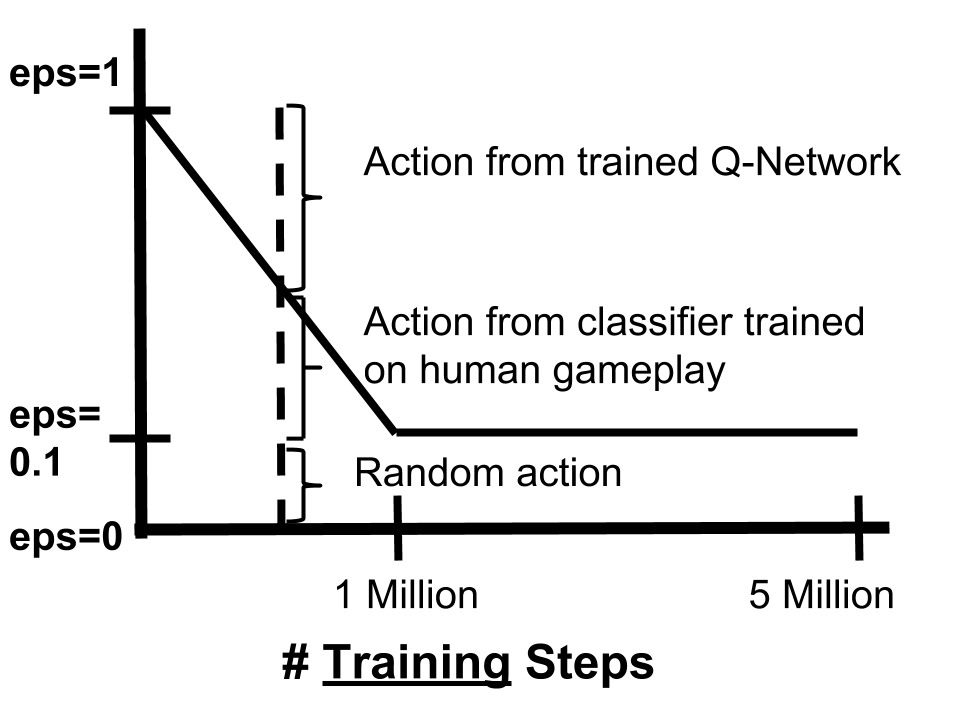
\includegraphics[width=0.45\textwidth]{figures/dqn_with_human_data_graph.png}
\caption{\footnotesize
TODO
}
\label{fig:human-guided-dqn}
\end{figure}

Fig.~\ref{fig:human-guided-dqn} presents a picture of the overall pipeline.

Due to the time-consuming aspects of this, we only perform with two games:
Breakout and Space Invaders, and leave other games to future work.

\subsection{Implementation Details}\label{ssec:implementation}

For coding purposes, we use a modified version of the
ALE~\cite{bellemare13arcade} which allows the human player to collect data. 

Describe preprocessing steps, etc.

Our classifier's code and supporting documents are
open-source.\footnote{\url{https://github.com/DanielTakeshi/Algorithmic-HRI}}

Our code is open-source and visible on
GitHub.\footnote{\url{https://github.com/DanielTakeshi/deep_q_rl}}

For additional details, see Appendix~\ref{app:preprocessing_details}.



%%%%%%%%%%%%%%%%%%%%%%%%%%%%%%%%%%%%%%%%%%%%%%%%%%%%%%%%%%%%%%%%%%%%%%%%%%%%%%%%
\section{Results: Human Gameplay}\label{sec:results_p1}

For additional details, see Appendix~\ref{app:experiment_details_human}.

IN PROGRESS

\subsection{Classifier Performance}

Discuss Breakout, Space Invaders results here, put a table here with the tuned
parameters?.

\begin{table}[!t]
\renewcommand{\arraystretch}{1.3}
\caption{Classifier Performance: Breakout}
\label{tab:breakout}
\centering
\begin{tabular}{c c c c | c c c c}
\hline
Reg. & $\lambda$ & Train & Valid & Reg. & $\lambda$ & Train & Valid \\
\hline
$L_1$ & 0.005 & 86.5 & 86.5 & $L_2$ & 0.005 & 86.5 & 86.5 \\
$L_1$ & 0.005 & 86.5 & 86.5 & $L_2$ & 0.005 & 86.5 & 86.5 \\
$L_1$ & 0.005 & 86.5 & 86.5 & $L_2$ & 0.005 & 86.5 & 86.5 \\
$L_1$ & 0.005 & 86.5 & 86.5 & $L_2$ & 0.005 & 86.5 & 86.5 \\
$L_1$ & 0.005 & 86.5 & 86.5 & $L_2$ & 0.005 & 86.5 & 86.5 \\
\hline
\end{tabular}
\end{table}

\begin{table}[!t]
\renewcommand{\arraystretch}{1.3}
\caption{Classifier Performance: Space Invaders}
\label{tab:space_invaders}
\centering
\begin{tabular}{c c c c | c c c c}
\hline
Reg. & $\lambda$ & Train & Valid & Reg. & $\lambda$ & Train & Valid \\
\hline
$L_1$ & 0.005 & 86.5 & 86.5 & $L_2$ & 0.005 & 86.5 & 86.5 \\
$L_1$ & 0.005 & 86.5 & 86.5 & $L_2$ & 0.005 & 86.5 & 86.5 \\
$L_1$ & 0.005 & 86.5 & 86.5 & $L_2$ & 0.005 & 86.5 & 86.5 \\
$L_1$ & 0.005 & 86.5 & 86.5 & $L_2$ & 0.005 & 86.5 & 86.5 \\
$L_1$ & 0.005 & 86.5 & 86.5 & $L_2$ & 0.005 & 86.5 & 86.5 \\
\hline
\end{tabular}
\end{table}

\subsection{Classifier Investigation}

Now provide example images?

\begin{figure*}[t]
\centering

\includegraphics[width=0.30\textwidth]{figures/empty.png}
\caption{\footnotesize
This will represent examples of game frames (i.e. sequence of 4 game frames) for
classifier, just like I did in the presentation. I'll want the full width (i.e.
two columns) for this, with good and bad examples from each game. More details
should be provided in a table with tuned values.
}
\label{fig:empty1}
\end{figure*}



%%%%%%%%%%%%%%%%%%%%%%%%%%%%%%%%%%%%%%%%%%%%%%%%%%%%%%%%%%%%%%%%%%%%%%%%%%%%%%%%
\section{Results: Modified DQN}\label{sec:results_p2}

For additional details, see Appendix~\ref{app:experiment_details_dqn}.

IN PROGRESS

\begin{figure*}[t]
\centering

\includegraphics[width=0.30\textwidth]{figures/empty.png}
\caption{\footnotesize
This will be another full-page figure. Here I'll hope to have the plots
comparing my results with DQN results, with both action-value and rewards. Use
moving averages. I may need a second one of these.
}
\label{fig:empty2}
\end{figure*}




%%%%%%%%%%%%%%%%%%%%%%%%%%%%%%%%%%%%%%%%%%%%%%%%%%%%%%%%%%%%%%%%%%%%%%%%%%%%%%%%
\section{Conclusions}\label{sec:conclusions}

In this work, we have made efforts to use Learning from Demonstration techniques
to boost the performance of DQN agents on the problem of playing Atari games. We
collected many hours of human expert gameplay data on Breakout and Space
Invaders, and provided extensive evidence to show that a convolutional
neural network can, to a large extent predict the action of the human expert
given a sequence of game frames. A DQN agent then used this classifier as part
of our human-guided DQN algorithm. While the DQN results do not improve using
our algorithm, we believe there is still potential for algorithmic improvements
in this work. In future work, we will first run the algorithm with a larger
number of exploration steps to better see the effects of the DQN agent. Second,
we will try the concept of \emph{human experience replay} and combine experience
replay from the agent's exploration with that of a human. Third, our more
elaborate goal is to shift gears and work on training attention
models~\cite{NIPS2014_5542,icml2015_xuc15}, the idea being that for these games,
there are only a few important signals that matter for score (e.g., is the ball
near the paddle in Breakout \emph{and} moving downwards?), and this can be
trained into an attention model. We will explore these directions of work in the
coming months.



\bibliographystyle{abbrv}
\bibliography{Daniel_Seita_Report_AHRI}

\appendices

\section{Preprocessing Details}\label{app:preprocessing_details}

We modify ALE so that a human player can play the games. This will
    create several directories inside (...)
    which is a folder that will have the \texttt{actions.txt},
    \texttt{rewards.txt} (per frame, not cumulative), and a \texttt{screenshots}
    folder that contains \emph{every} frame in the game, which is 60 per
    seconds. That's a lot of data, and it's in the raw RGB format as well, in
    \texttt{(210,160,3)} dimensions.  Then I (personally) will play Pong or
    Breakout (one simple game to start) for, I guess, maybe 5-6 hours to gather
    a crapload of data. I can do the same for other games.

Next, with all this raw data, we have to process it somehow. I will
    have another script that can do all of this at once. My guess is to pass it
    a parameter $k$ (say $k=4$) so that it combines $k$ consecutive frames
    together, thus reducing the number of files by a factor of $k$ (but each
    file itself is larger by a factor of $k$ so the overall size is the same).

Now we can get to our real contributions. The first one will be to
    develop a simple classifier from game frames to actions. There are several
    issues we have to get around regarding what frames to skip, though. Here is
    what I think I know:

    \begin{itemize}
        \item The ALE environment will process all frames (so 60fps really means
        60 frames per second!) by default, so if I want to use all frames, I can
        do that!

        \item Frame skip? This means skipping frames at the ALE level, so with
        ``game ticks'' which are the \emph{real}, single-frame case, we end up
        only considering $\{t_0, t_4, t_8, \ldots \}$ to be used for $\phi$. See
        John Schulman's description after this.

        \item Phi history? Recall that most say they use $\phi(s)$ to be the
        ``last four frames'' so the input to the CNN is $84 \times 84 \times 4$
        (I \emph{assume} the actions are ignored.) Ah, yes! Look
        at\footnote{https://github.com/openai/gym/issues/275} John
        Schulman's explanation: \emph{You can stack the frames returned by the
        environment That's the same thing done in the other papers that use the
        Atari domain, such as deepmind's paper.  I.e., they stack frames (t,
        t-4, t-8, t-12), not (t,t-1,t-2,t-3).} This really helps! So now I know
        that $\phi$ is the last $m$ (where $m=4$ usually) game frames,
        \emph{when only considering the non-skipped frames}. Got
        it.\footnote{All of this should be in a blog post someday.}

        \item OpenAI environments automatically repeat actions for 2, 3, or 4
        frames (at random). So instead of $\{t_0,t_4,t_8,\ldots\}$, we could get
        $\{t_0,t_3,t_7,t_9,\ldots\}$. I see! This introduces more stochasticity.
        Maybe this no longer needs the human starts condition?

        \item The original DQN paper (I think both NIPS and NATURE versions?)
        used frame skipping with max values attached to \emph{consecutive}
        frames, and this time consecutive really means consecutive! It includes
        skipped frames. Ouch! In other words, the input to the neural network
        is, I believe:
        \begin{verbatim}
        [max(T-1, T), max(T-3, T-4), max(T-7, T-8), max(T-11, T-12)]
        \end{verbatim}
        So one of those above is a $\phi(s_T)$ that is our state. Looks like no
        actions here. And also, these are the units of information that get
        stored in the experience replay ... along with actions and rewards,
        which I \emph{guess} are the action and reward at the same frame as $T$,
        but not sure, seems like it would be better to have it a few frames
        \emph{after} $T$.

        \item Details on the database for experience replay: these should be of
        the form $(s,a,r,s')$, but what exactly are the components?
    \end{itemize}

    What does this mean in practice for me? When I play the games, I get
    screenshots, actions and rewards \emph{every} time step. So how do I gather
    the data?

\begin{itemize}
        \item First, we develop a series of indices which we want to use, i.e.
        generate via numpy an array that looks like:
        \begin{verbatim}
        [0,3,7,9,11,15,19,22,26,...]
        \end{verbatim}
        and then only extract the data from those indices. That will
        automatically reduce the number of frames by a factor of 2-4 (the reason
        why I use 2,3,4 is because that's what OpenAI uses). Then subsample
        actions and rewards using those exact indices (should be OK, rewards and
        actions come right after those state indices). Then after this is done,
        downsample the remaining screenshots to 84x84 pixels. This \emph{will}
        be game-dependent!

        \item After reading open-sourcer DQN code, it indeed looks like
        $\phi(s_t)$ and $\phi(s_{t+1})$ (i.e. $s$ and $s'$ in normal MDP
        notation) share (non-skipped) frames. That is, for the example above, I
        will need to make $\phi(s_0) = (x_0,x_3,x_7,x_9)$ where $x_i$ denotes
        the screenshots at \emph{time-step} $i$, \emph{including} skipped frames
        Then $\phi(s_1) = (x_3,x_7,x_9,x_{11})$. The action $a$ and reward $r$
        for this particular sample are chosen according to action $a_9$ and
        $r_9$ at time-step 9 according to the last one in $\phi(s_0)$. All this
        will be repeated to form $(\phi(s_t),a_t,r_t,\phi(s_{t+1}))$.

        \item And \emph{that} is the dataset which we can put in for the
        experience replay rule. I will save all of this in separate folders, but
        combining all the games together. This is following the reference which
        uses human experience replay.

        \item OK, but what about training a classifier from images to actions?
        For this, I believe we want to gather all the $(\phi(s_t),a_t)$ and
        simply use that. Alternatively, I can try $(\phi(s_t),a_{t+k})$ for some
        \emph{small} value $k$ (remember, there's frame skipping, and I feel
        like this won't make that much of a difference). Then I train on that to
        get a classifer. How to use it? During the exploration phase where we're
        following random actions with probability $\epsilon$, simply follow what
        the classifier tells us to do. This is \emph{different} from the human
        experience replay technique (but it can be combined with it!).
\end{itemize}

\section{Experiment Details}\label{app:experiment_details}

TODO

\subsection{Human Gameplay Classifier}\label{app:experiment_details_human}

TODO

\subsection{Deep Q-Network With Human Data}\label{app:experiment_details_dqn}

TODO

\end{document}

% Daniel: this might be useful.

% An example of a double column floating figure using two subfigures.
% (The subfig.sty package must be loaded for this to work.)
% The subfigure \label commands are set within each subfloat command,
% and the \label for the overall figure must come after \caption.
% \hfil is used as a separator to get equal spacing.
% Watch out that the combined width of all the subfigures on a 
% line do not exceed the text width or a line break will occur.
%
%\begin{figure*}[!t]
%\centering
%\subfloat[Case I]{\includegraphics[width=2.5in]{box}%
%\label{fig_first_case}}
%\hfil
%\subfloat[Case II]{\includegraphics[width=2.5in]{box}%
%\label{fig_second_case}}
%\caption{Simulation results for the network.}
%\label{fig_sim}
%\end{figure*}
%
% Note that often IEEE papers with subfigures do not employ subfigure
% captions (using the optional argument to \subfloat[]), but instead will
% reference/describe all of them (a), (b), etc., within the main caption.
% Be aware that for subfig.sty to generate the (a), (b), etc., subfigure
% labels, the optional argument to \subfloat must be present. If a
% subcaption is not desired, just leave its contents blank,
% e.g., \subfloat[].


% An example of a floating table. Note that, for IEEE style tables, the
% \caption command should come BEFORE the table and, given that table
% captions serve much like titles, are usually capitalized except for words
% such as a, an, and, as, at, but, by, for, in, nor, of, on, or, the, to
% and up, which are usually not capitalized unless they are the first or
% last word of the caption. Table text will default to \footnotesize as
% the IEEE normally uses this smaller font for tables.
% The \label must come after \caption as always.
%
%\begin{table}[!t]
%% increase table row spacing, adjust to taste
%\renewcommand{\arraystretch}{1.3}
% if using array.sty, it might be a good idea to tweak the value of
% \extrarowheight as needed to properly center the text within the cells
%\caption{An Example of a Table}
%\label{table_example}
%\centering
%% Some packages, such as MDW tools, offer better commands for making tables
%% than the plain LaTeX2e tabular which is used here.
%\begin{tabular}{|c||c|}
%\hline
%One & Two\\
%\hline
%Three & Four\\
%\hline
%\end{tabular}
%\end{table}
